\documentclass[12pt,fleqn]{article}\usepackage{../../common}
\begin{document}
Katı-Gövde Simülasyonu

Dönüş Animasyonu

Bir örnek gövde üzerinde simülasyon yapmaya uğraşalım. Elimizde bir simit, ya da
geometride torus denen bir şekil var. Bu dosya STL denen bir format içinde,
detaylar için [1]. Kuvvet uygulama sonrası lineer ve açısal momentum içeren
simülasyon için pek çok değişkeni diferansiyel tanımları üzerinden entegre
etmemiz gerekiyor, daha basit bir örnek ile, özellikle sabit bir açışal hız
üzerinden salt döndürme ile başlamak uygun olabilir. [4]'te tarif edilen
döndürme matrisi türevini hatırlarsak,

$$
\frac{\ud R}{\ud t} = \tilde \omega \cdot R
$$

Döndürmeyi bir $\omega$ etrafında düşünüyorduk, $\omega$'nin büyüklüğü
açısal dönme hızına tekabül ediyordu, ve $\tilde \omega$ eksi-bakışımlı
matris idi.

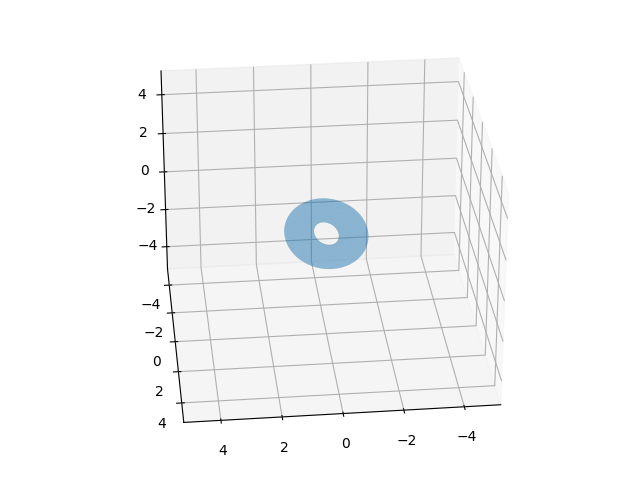
\includegraphics[width=25em]{phy_005_basics_04_01.png}

Tüm bunları entegre edici \verb!odeint! çağrısının kabul edeceği bir formda
nasıl kullanırız? Bu çağrı düzleştirilmiş bir liste içinde diferansiyel
sonuçların, ve ana değişkenlerin olmasını bekliyor. O zaman $R$'yi kolon bazlı
olmak üzere düzleştiririz, ve gerektiği o listeden matris formuna geçeriz, vs.

\begin{minted}[fontsize=\footnotesize]{python}
from scipy.integrate import odeint
from stl import mesh

def skew(a):
   return np.array([[0,-a[2],a[1]],[a[2],0,-a[0]],[-a[1],a[0],0]])

your_mesh = mesh.Mesh.from_file('torus.stl')
prop = your_mesh.get_mass_properties()
R0 = np.eye(3,3)
omega = np.array([1.0,1.0,1.0])
#omega = np.array([0.0,1.0,0.0])
skew_omega = skew(omega)
   
def dRdt(u,t):   
   R1x,R1y,R1z,R2x,R2y,R2z,R3x,R3y,R3z = u
   R = np.array([R1x,R1y,R1z,R2x,R2y,R2z,R3x,R3y,R3z])
   R = R.reshape((3,3)).T
   res = np.dot(skew_omega, R)
   return list(res.T.flatten())

LIM = 5
STEPS = 20
t=np.linspace(0.0, 3.0, STEPS)
R0 = np.eye(3,3)
u0 = R0.flatten()
u1=odeint(dRdt,list(u0),t)
\end{minted}

Üstte görülen mesela \verb!R1x! $R$ matrisinin 1'inci kolonunun $x$ değişkeni
anlamında.

Simülasyonda simit şeklinin baktığı yön $R$ içinde, ve grafik amaçlı olarak her
seferinde simit şeklini sıfırdan yükleyip son $R$'ye ilerletiyoruz, ve her
adımda bu grafiği basıyoruz.  Simülasyonu hesapladık, tüm sonuç \verb!u1!
içinde, görüntüden bazı seçilmiş kareler altta görülebilir,

\begin{minted}[fontsize=\footnotesize]{python}
import matplotlib.pyplot as plt
from mpl_toolkits import mplot3d

def plot_vector(fig, orig, v, color='blue'):
   ax = fig.gca(projection='3d')
   orig = np.array(orig); v=np.array(v)
   ax.quiver(orig[0], orig[1], orig[2], v[0], v[1], v[2],color=color)
   ax = fig.gca(projection='3d')  
   return fig

for i in range(STEPS):
    fig = plt.figure()
    axes = mplot3d.Axes3D(fig)
    your_mesh = mesh.Mesh.from_file('torus.stl')
    R = u1[i].reshape((3,3)).T
    your_mesh.rotate_using_matrix(R)
    scale = your_mesh.points.flatten()
    axes.add_collection3d(mplot3d.art3d.Poly3DCollection(your_mesh.vectors,alpha=0.3))
    plot_vector(fig, [0,0,0], omega, color='red')
    axes.auto_scale_xyz(scale, scale, scale)
    axes.set_xlim(-LIM,LIM);axes.set_ylim(-LIM,LIM);axes.set_zlim(-LIM,LIM)
    axes.view_init(azim=20,elev=0)
    plt.savefig('/tmp/rotate_%02d.png' % i)  
\end{minted}

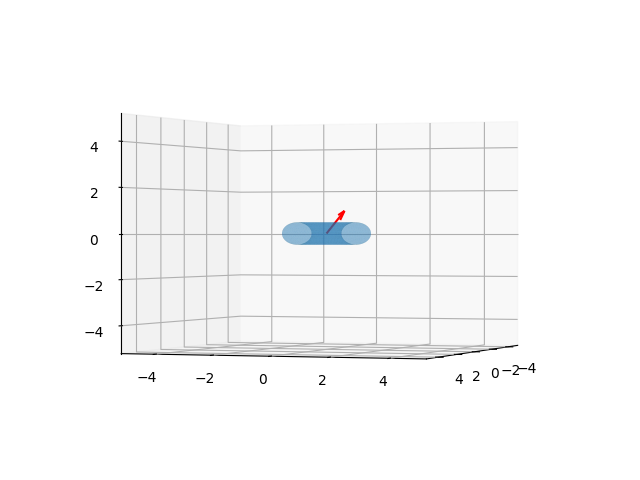
\includegraphics[width=20em]{sim1/rotate_00.png}

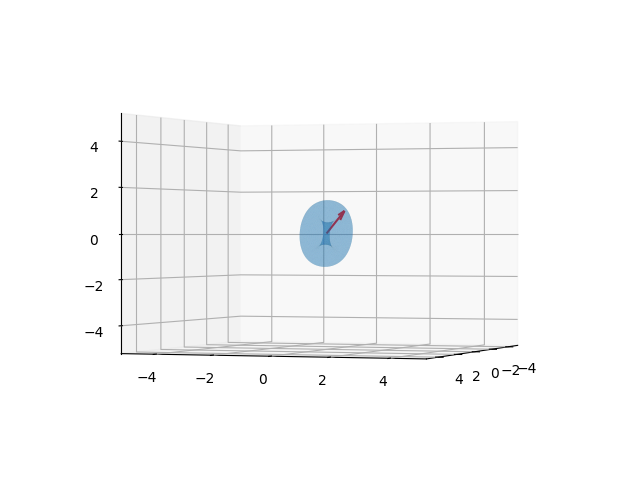
\includegraphics[width=20em]{sim1/rotate_08.png}

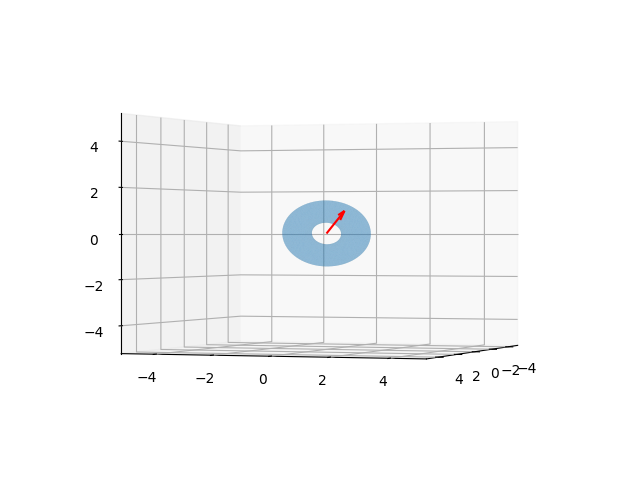
\includegraphics[width=20em]{sim1/rotate_14.png}

\begin{minted}[fontsize=\footnotesize]{python}
! convert -delay 20 -loop 0 /tmp/rotate*.png /tmp/rotate1.gif
\end{minted}

Animasyon sonucu [4]'te bulunabilir.

Torus şekli hakkında bazı istatistikler alttadır.

\begin{minted}[fontsize=\footnotesize]{python}
from stl import mesh

your_mesh = mesh.Mesh.from_file('torus.stl')

prop = your_mesh.get_mass_properties()
print ('hacim',np.round(prop[0],3))
print ('yercekim merkezi (COG)',np.round(prop[1],3))
print ('COG noktasinda atalet matrisi')
print (np.round(prop[2],3))
\end{minted}

\begin{verbatim}
hacim 4.918
yercekim merkezi (COG) [-0.  0. -0.]
COG noktasinda atalet matrisi
[[ 3.223 -0.     0.   ]
 [-0.     3.223  0.   ]
 [ 0.     0.     5.832]]
\end{verbatim}

COG'nin sıfır noktasında olması mantıklı çünkü STL dosyasında simit şekli oraya
konmuş, ve simit şekli simetrik bir şekil.

%<a name='full'/>

İttirme Animasyonu

Bu animasyon için katı gövdeye bir noktada bir kuvvet uyguluyacağız. O noktayı
seçmek için STL formatında olan üçgenlerden birini kullanabiliriz, çünkü bu
üçgenlerin gövdenin yüzeyinde bir yerlerde olduğunu biliyoruz, Torus STL şekli
bu üçgenlerin herbirine dik olan normal vektörü STL formatında zaten, o
üçgenlerden birinin normal vektörünü ters çevirirsek, o noktaya o yönde bir
kuvvet uyguladığımızı hayal edebililriz, ve simülasyonun geri kalanını bu
noktadan devam ettiririz.

\begin{minted}[fontsize=\footnotesize]{python}
import matplotlib.pyplot as plt
from mpl_toolkits import mplot3d

fig = plt.figure()
axes = mplot3d.Axes3D(fig)

SCALE = 4
LIM = 5

scale = your_mesh.points.flatten()
axes.add_collection3d(mplot3d.art3d.Poly3DCollection(your_mesh.vectors,alpha=0.3))
axes.auto_scale_xyz(scale, scale, scale)

def plot_vector(fig, orig, v, color='blue'):
   ax = fig.gca(projection='3d')
   orig = np.array(orig); v=np.array(v)
   ax.quiver(orig[0], orig[1], orig[2], v[0], v[1], v[2],color=color)
   ax = fig.gca(projection='3d')  
   return fig

axes.set_xlim(-LIM,LIM);axes.set_ylim(-LIM,LIM);axes.set_zlim(-LIM,LIM)

tidx = 2000
o = np.mean(your_mesh.vectors[tidx],axis=0)
axes.plot (o[0],o[1],o[2],'gd')
n = your_mesh.get_unit_normals()[tidx]
plot_vector(fig, o, n*SCALE)
plot_vector(fig, o, -n*SCALE, color='red')
axes.view_init(azim=84,elev=28)

plt.savefig('phy_005_basics_04_05.png')
\end{minted}

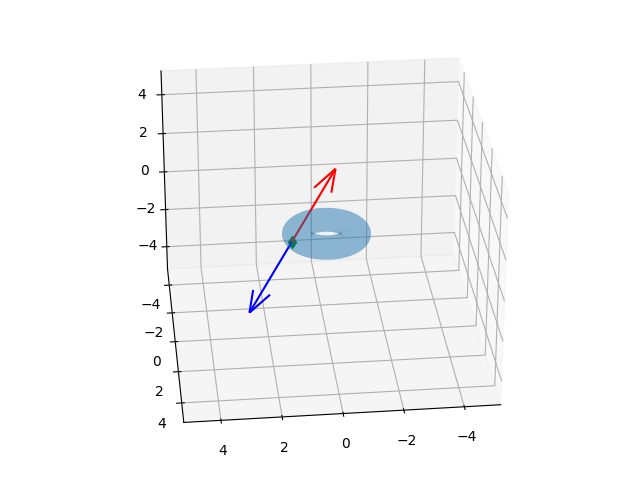
\includegraphics[width=20em]{phy_005_basics_04_05.png}

Kuvveti kırmızı vektörle gösterilen yönde uygulayabiliriz.

Şimdi ``sıfırıncı anda'' yani ilk başlangıçta uygulanan kuvvetleri, lineer,
açısal, hesaplamak lazım. Noktayı üstte seçtik, sonu o noktada başlangıcı nesne
ağırlık merkezinde olan bir vektör ile kuvvet vektörü arasında çapraz çarpım
yapıyoruz, bu bize torku veriyor.

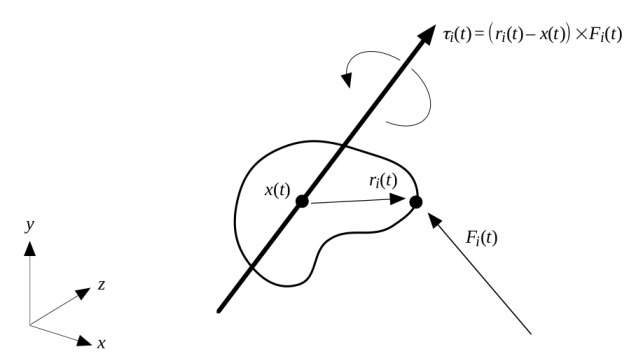
\includegraphics[width=25em]{phy_008_sim_rigbod_01.png}

Benzer şekilde sonu nesne merkezinde başı o noktada olan bir vektör daha var,
lineer kuvvet bu doğrultuda uygulanacak, o vektör üzerine iki üstte görülen
kırmızı vektörü yansıtıyoruz, bu da lineer kuvvet oluyor. Bir üstteki resim
üzerinde gösterirsek,

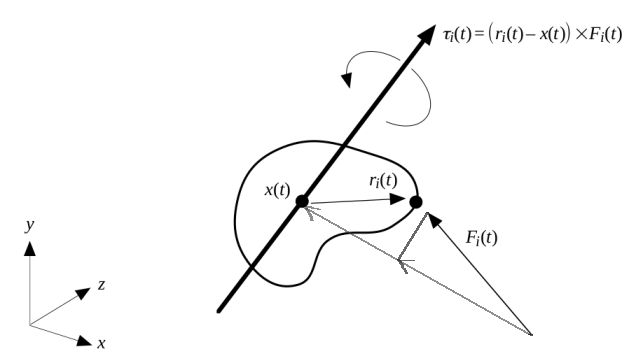
\includegraphics[width=25em]{phy_008_sim_rigbod_02.png}

Daha önce söylediğimiz gibi her iki kuvvet de ilk anda lineer ve açısal
momentumu ekileyen faktörler, sonraki adımlarda etkileri yok.

Ayrıca entegrasyon için kendi pişirdiğimiz kodları kullanacağız, \verb!odeint!
işleri zorlaştırabilir çünkü zamana bağlı bazı farklı kodlamalar var, ayrıca
$I^{-1}$ her adımda sürekli değişiyor, yani bir konum güncellemesi var, bu
tür kodlamalar kapalı bir kutu isteyen \verb!odeint! ile daha zor olabilir.
Bunlar problem değil, [5]'te paket kullanmadan hesaplanan bir
kodlama şeklini görmüştük.

\begin{minted}[fontsize=\footnotesize]{python}
import numpy as np
from stl import mesh
import numpy.linalg as lin

your_mesh = mesh.Mesh.from_file('torus.stl')   
prop = your_mesh.get_mass_properties()
cog = np.round(prop[1],3) # baslangic aninda obje COG
Ibody = np.round(prop[2],3)
Ibodyinv = lin.inv(Ibody)
dt = 0.1
x = np.zeros((1,3))
R = np.eye(3,3)
L = np.zeros((1,3))
v = np.zeros((1,3))
F = np.zeros((3,1))
M = 1
P = M*v

def skew(a):
   return np.array([[0,-a[2],a[1]],[a[2],0,-a[0]],[-a[1],a[0],0]])

tidx = 2000
apply_at = np.mean(your_mesh.vectors[tidx],axis=0) - cog
f_at = -1 * 5 * your_mesh.get_unit_normals()[tidx]
tau0 = np.cross(apply_at, f_at).reshape(1,3) * 10.0
flindir = cog-apply_at
flin0 = np.dot(f_at,flindir)*(flindir/np.abs(lin.norm(flindir)))

res = []
for i in range(30):
   xold,Rold,Pold,Lold = x.copy(),R.copy(),P.copy(),L.copy()
   
   Iinv = np.dot(np.dot(Rold, Ibodyinv), Rold.T)
   omega = np.dot(Iinv, Lold.T).T
   omega = omega.reshape(3)
   skew_omega = skew(omega)
   R = Rold + np.dot(skew_omega, Rold) * dt

   v = Pold / M
   x = x + v*dt
   P = Pold
   if i==0: # baslangic ani
      L = Lold + tau0*dt
      P = Pold + (flin0*dt)
   else:      
      L = Lold # sonraki adimlarda degisim yok
      P = Pold # momentum ayni kaliyor
   res.append([x,R,P,L])
\end{minted}

Hesaplar yapıldı, şimdi grafikleme,

\begin{minted}[fontsize=\footnotesize]{python}
import matplotlib.pyplot as plt
from mpl_toolkits import mplot3d

LIM = 5
SCALE = 4

def plot_vector(fig, orig, v, color='blue'):
   ax = fig.gca(projection='3d')
   orig = np.array(orig); v=np.array(v)
   ax.quiver(orig[0], orig[1], orig[2], v[0], v[1], v[2],color=color)
   ax = fig.gca(projection='3d')  
   return fig

for i, [x,R,P,L] in enumerate(res):
   fig = plt.figure()
   axes = mplot3d.Axes3D(fig)
   your_mesh = mesh.Mesh.from_file('torus.stl')
   # t-0 aninda uygulanan kuvvet yonunu goster
   o = np.mean(your_mesh.vectors[tidx],axis=0)
   n = your_mesh.get_unit_normals()[tidx]
   plot_vector(fig, o, -n*SCALE, color='red')
   
   your_mesh.rotate_using_matrix(R)
   your_mesh.translate(x.reshape(3))
   scale = your_mesh.points.flatten()
   axes.add_collection3d(mplot3d.art3d.Poly3DCollection(your_mesh.vectors,alpha=0.3))
   axes.auto_scale_xyz(scale, scale, scale)
   axes.set_xlim(-LIM,LIM);axes.set_ylim(-LIM,LIM);axes.set_zlim(-LIM,LIM)

   az = 80-(i*2) # kamera dondurmek icin
   axes.view_init(azim=az,elev=28)
   plt.savefig('/tmp/rotate_%02d.png' % i)
   plt.close('all')    
\end{minted}

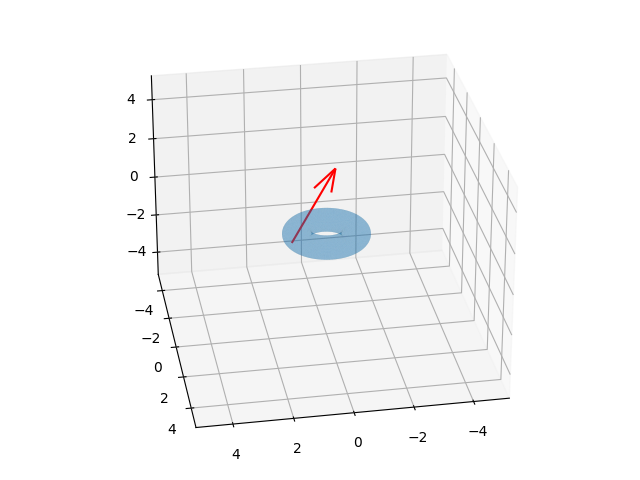
\includegraphics[width=20em]{sim2/rotate_00.png}
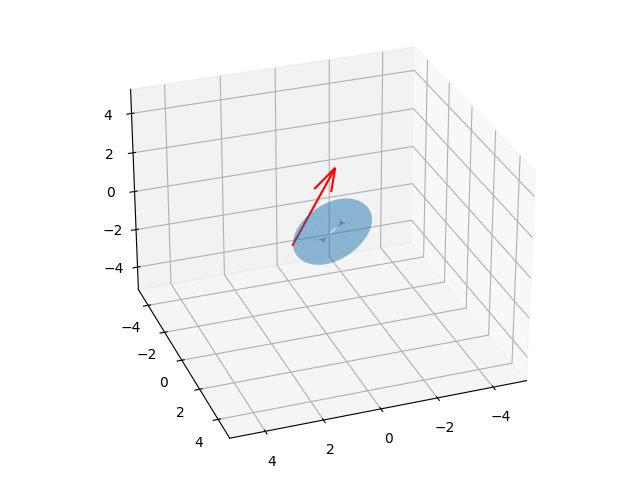
\includegraphics[width=20em]{sim2/rotate_05.png}

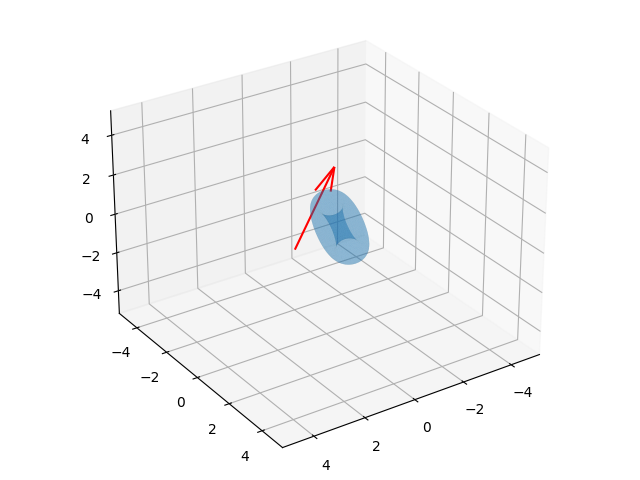
\includegraphics[width=20em]{sim2/rotate_12.png}
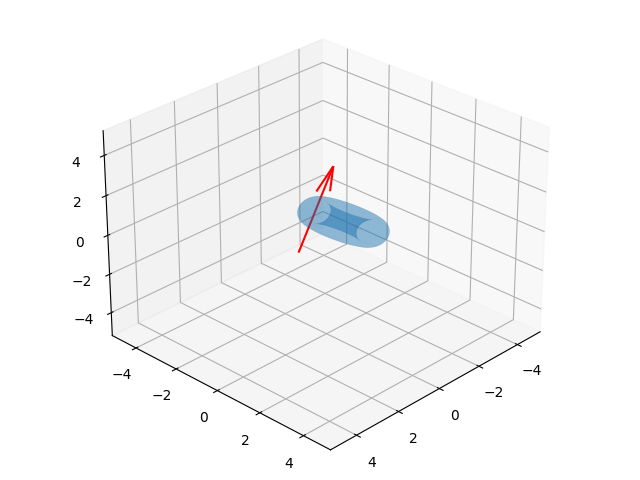
\includegraphics[width=20em]{sim2/rotate_18.png}


\begin{minted}[fontsize=\footnotesize]{python}
! convert -delay 20 -loop 0 /tmp/rotate*.png /tmp/rotate2.gif
\end{minted}

Animasyon sonucu [6]'da görülebilir. Hareket mantıklı gözüküyor, unutmayalım
grafikleme açısından kolay olduğu için öyle çizildi fakat aslında hesaplara göre
vektörün ucu kuvvet uygulanan noktada, ve uygulanan kuvvet sonrası şekil dönmeye
başlayarak ve yukarı doğru uçarak devam ediyor (kuvvet alttan yukarı doğru).
Simülasyon ortamı boşluk ortamı, uzay gibi yerçekimsiz bir yer, tek kuvvet ilk
başta şekle uygulanan kuvvet, ardından momentum muhafazası ile hareket devam
ediyor.

Kaynaklar

[1] Bayramlı, {\em 3D Baskıya Hazır CAD Tasarımlarına Erişmek, Numpy-STL},
    \url{https://burakbayramli.github.io/dersblog/sk/2020/08/numpy-stl.html}

[2] Witkin, {\em Physically Based Modeling}

[3] Bayramlı, {\em Animasyon 1},
    \url{https://drive.google.com/uc?export=view&id=17qlJvaucB6_l0eLUfcevu84qNXQocGHO}

[4] Bayramlı, {\em Fizik, Temel Fizik 4, Katı Gövde}

[5] Bayramlı, {\em Fizik, Simulasyon}

[6] Bayramlı, {\em Animasyon 2},
    \url{https://drive.google.com/uc?export=view&id=1ZvONRASb4By5zKnuDs6unAVwj0PA8_HK}

\end{document}



